\section{電源系 (概要/EPS/インヒビット設計(二重絶縁)/電源系統図/電池/SAP)(池谷・中塚)}
\subsection{概要}
本節では本衛星の電源系について述べる.本衛星の電源系の概要を図\ref{3_1_power_diagram}に示す.本衛星の電源系は主に以下のコンポーネントから構成されている.
\begin{itemize}
	\item 太陽電池パネル(Solar Array Panel, SAP)
	\item バッテリ
	\item CIB電源系
	\item 電源基板 (Electrical Power System, EPS)
	\item 伸展カメラ部電源系
\end{itemize}


% begin{landscape}
% begin{figure}[htbp]
% 	\begin{center}
% 		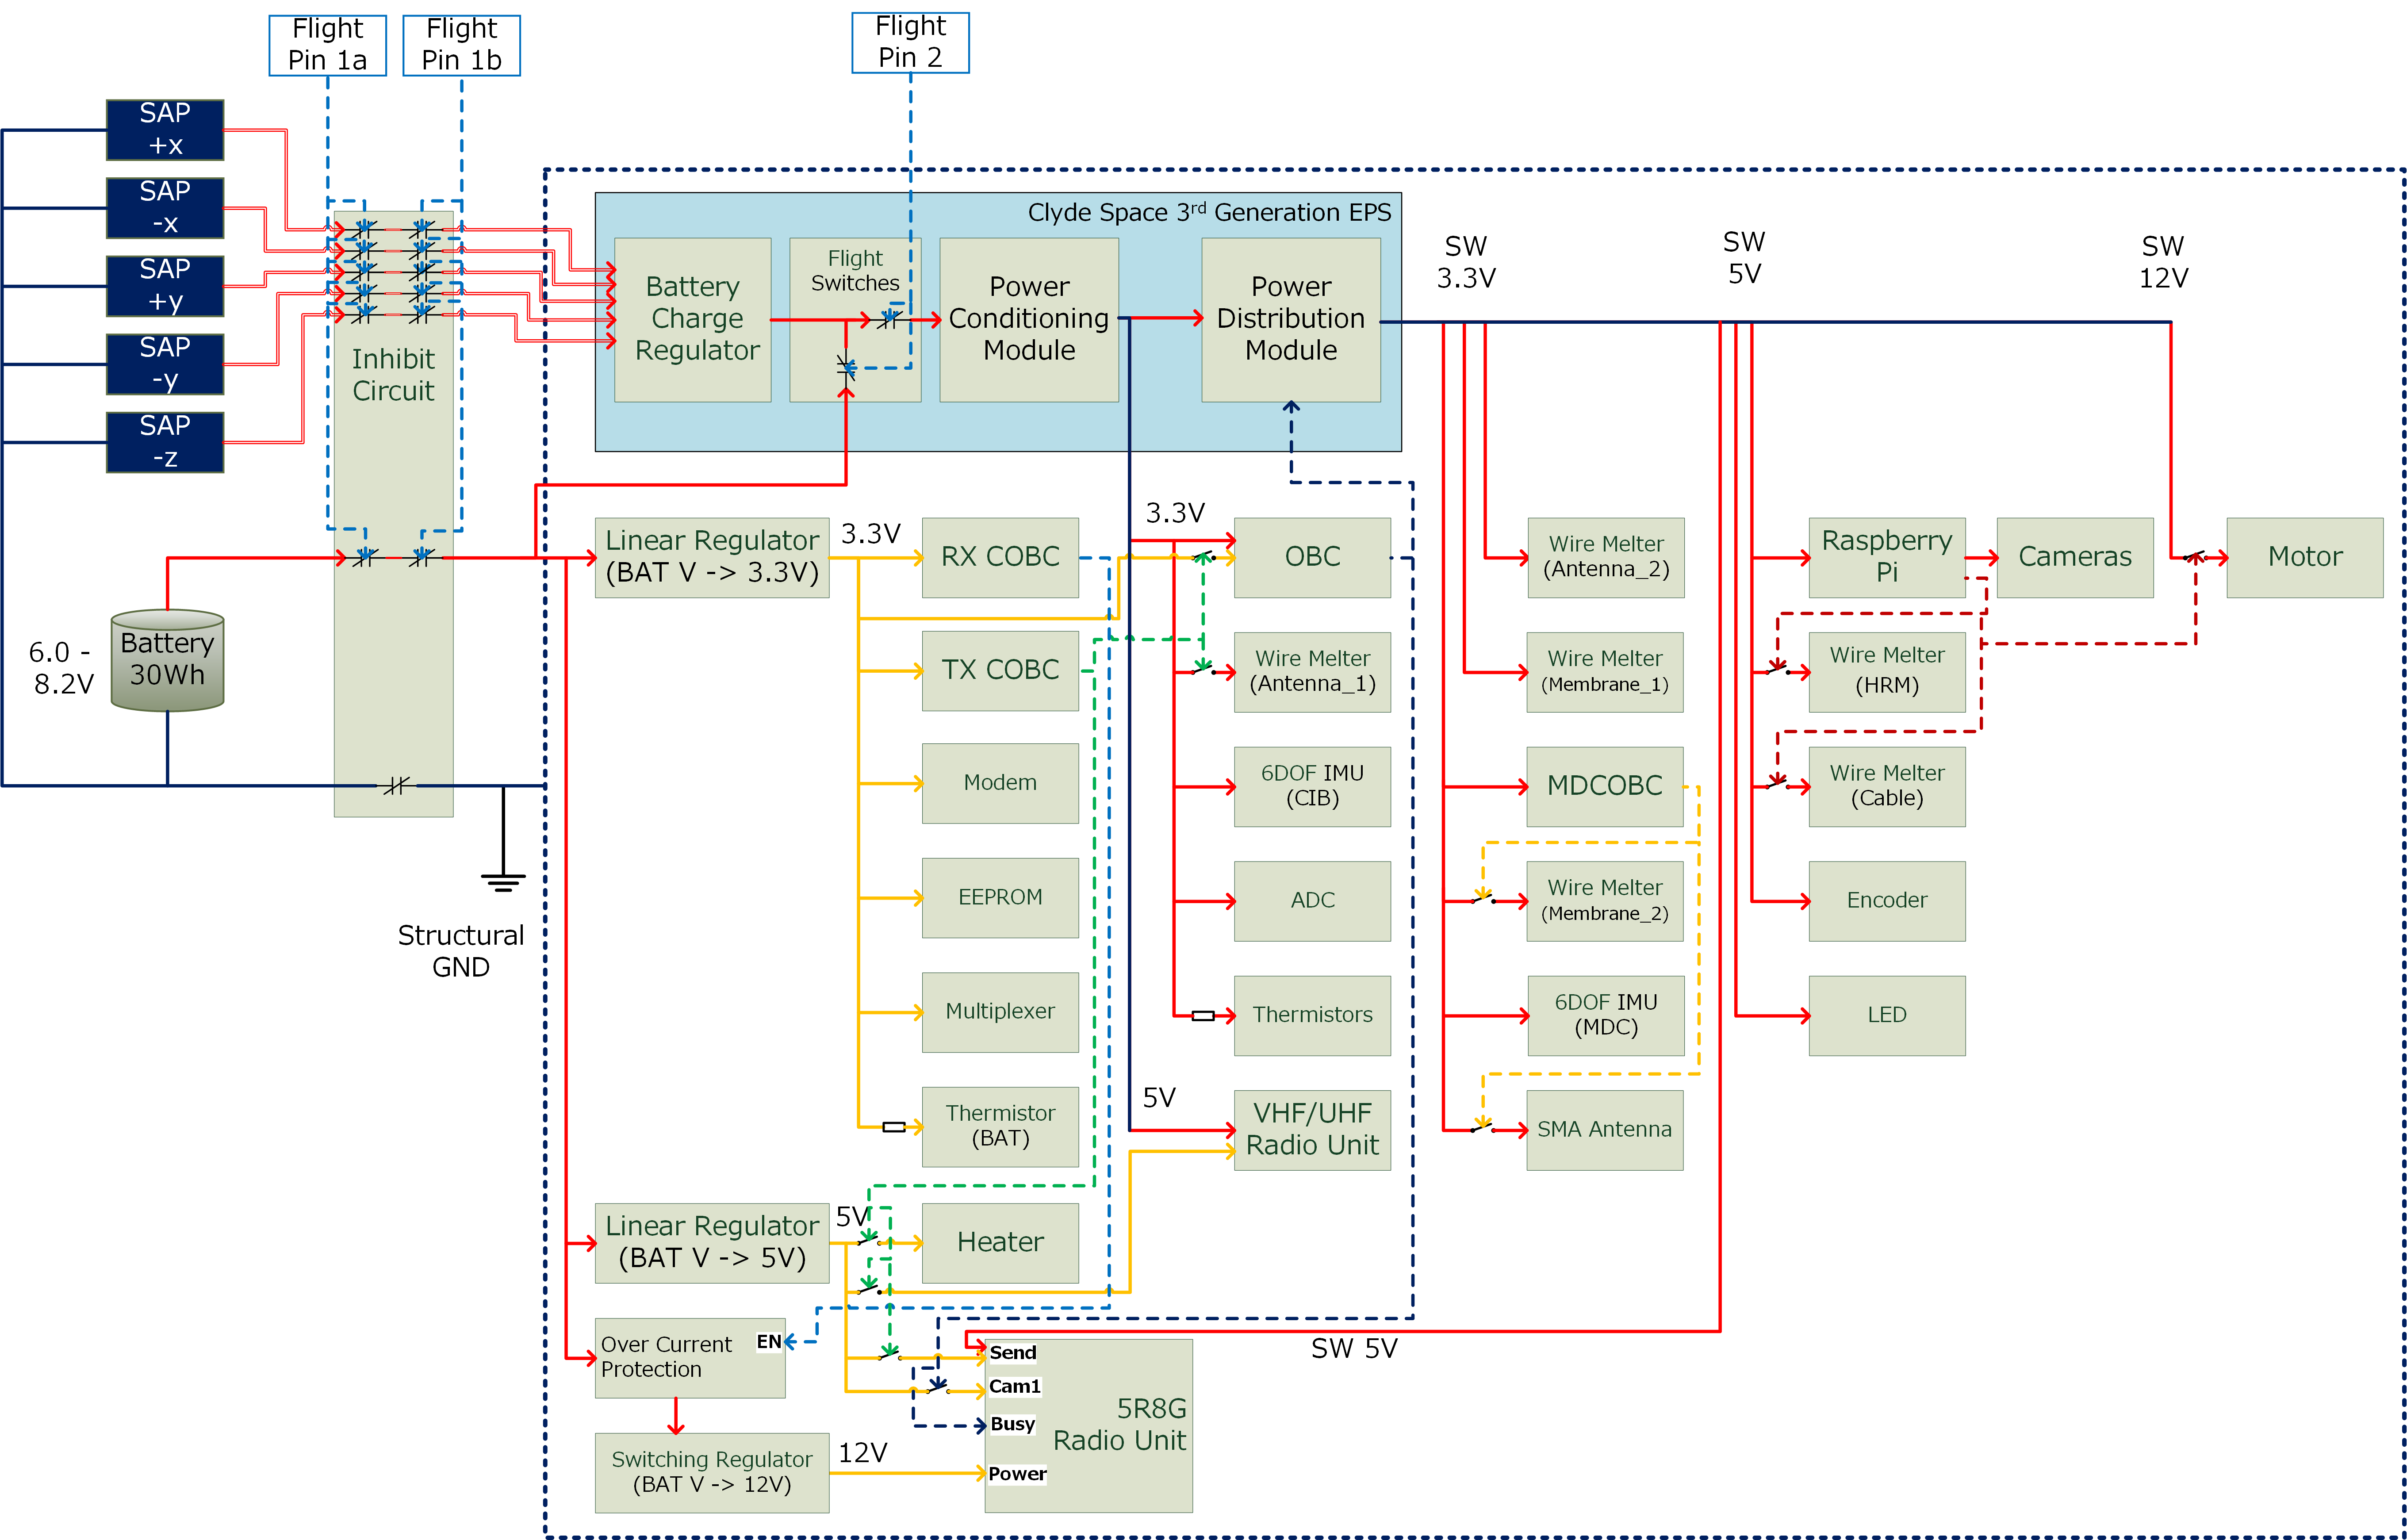
\includegraphics[width=0.5\linewidth]{./03/fig/Power_diagram.png}
%		\caption{Example of a figure caption.}
%		\label{3_1_power_diagram}
%	\end{center}
% \end{figure}
% \end{landscape}            


\subsection{SAP}

\subsubsection{SAP試験}

\subsection{バッテリ}
バッテリは公称電圧7.6V,放電容量3900mAhのClyde Space社の30Whr Standalone CubeSat Batteryを購入した(図\ref{fig3_1_bat}).バッテリの電気・構造的特性を表\ref{table3_1_bat_spec}に,絶対最大定格を表\ref{table3_1_bat_max}に示す.このバッテリパックは2直3並列(2S3P)のリチウムポリマー電池であり,UN勧告適合品,NASA標準EP-Wi-032適合品である.

\begin{figure}[htbp]
	\begin{center}
		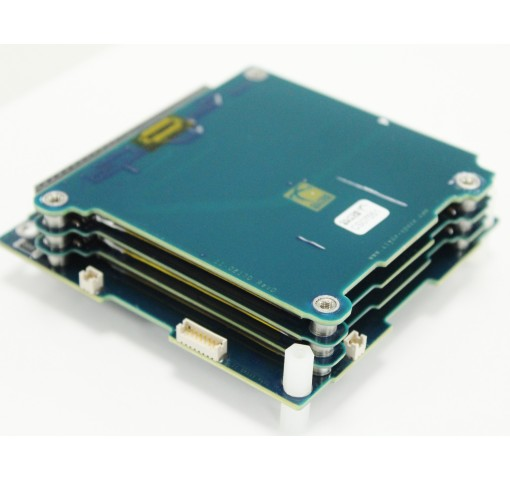
\includegraphics[width=0.5\linewidth]{./03/fig/battery.jpg}
		\caption{30Whr Standalone CubeSat Battery (c)Clyde Space}
		\label{fig3_1_bat}
	\end{center}
\end{figure}

\begin{table}[htbp]
	\begin{center}
		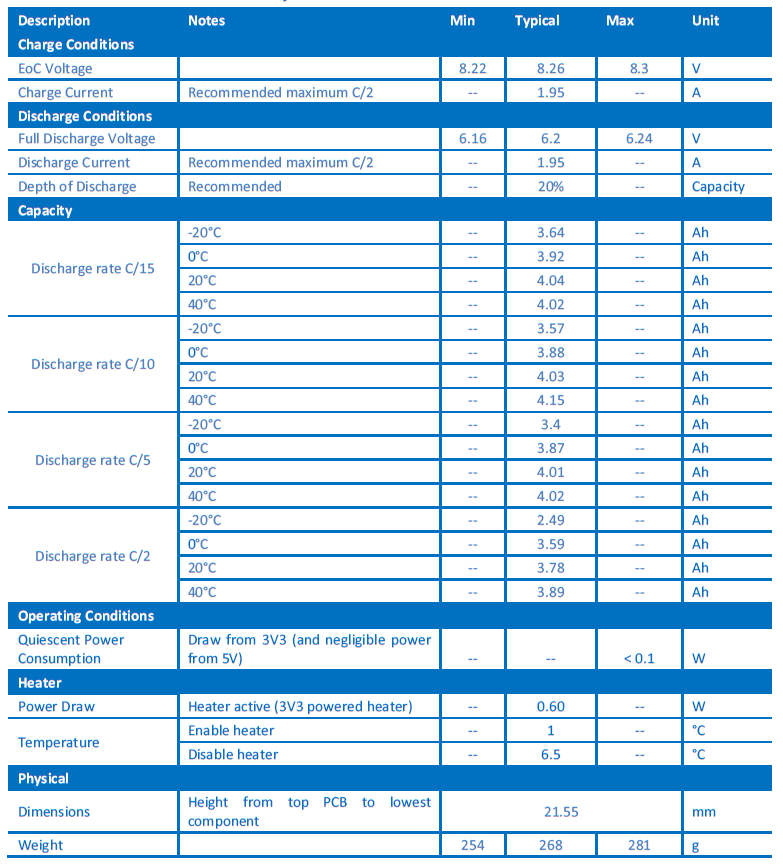
\includegraphics[width=0.9\linewidth]{./03/fig/battery_spec.png}
		\caption{30Whr}
		\label{table3_1_bat_spec}
	\end{center}
\end{table}


\begin{table}
	\caption{Maximum Ratings of the Battery}
	\label{table3_1_bat_max}
	\centering
	\begin{tabular}{ccccc}
		\hline \hline
		\multicolumn{5}{c}{Max Ratings Over Operating Temperature Range (Unless Otherwise Stated)}\\
		&&BCR  & Value  &  Unit  \\
		\hline
		\multirow{3}{*}{Charge Limits}&Voltage&max&8.4&V\\
		&Current&max&6&A\\
		&Current Rate& max &1.53C &Fraction of Capacity\\
		\hline
		\multirow{3}{*}{Discharge Limits}&Voltage&max&6.2&V\\
		&Current&max&6&A\\
		&Current Rate& max &1.53C &Fraction of Capacity\\
		\hline
		\multicolumn{2}{c}{Operating Temperature}&\multicolumn{2}{c}{ -10 to 50} & °C\\
		\multicolumn{2}{c}{\multirow{3}{*}{Storage Temperature}}&\multicolumn{2}{c}{1 Year: -20 to +20}&\multirow{3}{*}{°C}\\
		&&\multicolumn{2}{c}{3 Months: -20 to +45}&\\
		&&\multicolumn{2}{c}{1 Month: -20 to +60}&\\
		\multicolumn{2}{c}{Vacuum}&\multicolumn{2}{c}{10-5}&torr\\
		\multicolumn{2}{c}{Vibration}&\multicolumn{2}{c}{To [RD-3]}\\
		\hline
	\end{tabular}
\end{table}
	




本バッテリにはセルレベルの過電流,過充電,過放電保護回路,および1並列ごとの過電流保護回路が組み込まれている.これらの保護機能については,メーカーから試験報告書を入手し,さらに本衛星開発チームで環境試験(振動,衝撃)前後での充放電特性を測定した.

付録かな

ヒータが組み込まれており0℃以下で作用する.この機能は無効にすることもできた.さらに温度関係なく制御可能な自作ヒータを貼り付けた.

FMおよびEMにおいてはバッテリの$\mathrm{I^{2}C}$ラインの故障が生じたために,組み込まれていた機能としてのテレメトリ取得が不可能となった.バッテリの電圧,温度取得等の情報は別ラインで取得可能にしていた.


\begin{figure}[htbp]
	\begin{center}
		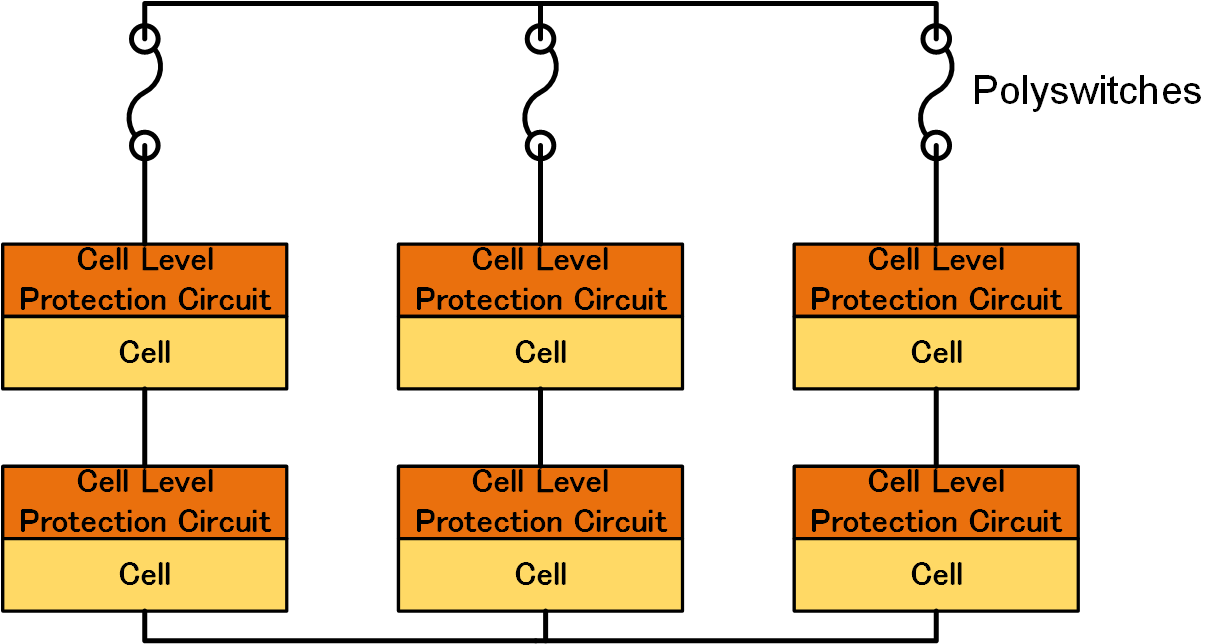
\includegraphics[width=0.5\linewidth]{./03/fig/BAT.png}
		\caption{Integrated EPS and Battery Protection Architecture 転載}
		\label{mir}
	\end{center}
\end{figure}

\begin{figure}[htbp]
	\begin{center}
		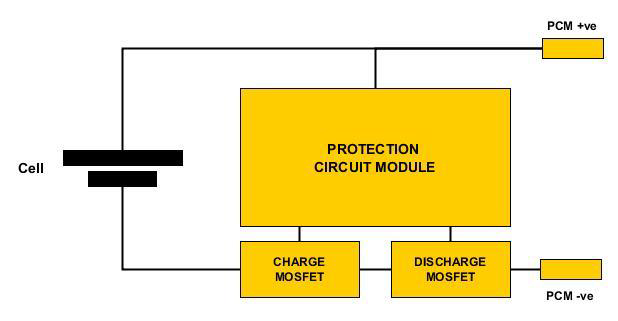
\includegraphics[width=0.5\linewidth]{./03/fig/cell_protection.png}
		\caption{Cell level protection circuit schematic 転載}
		\label{cell_p}
	\end{center}
\end{figure}

\begin{figure}[htbp]
	\begin{center}
		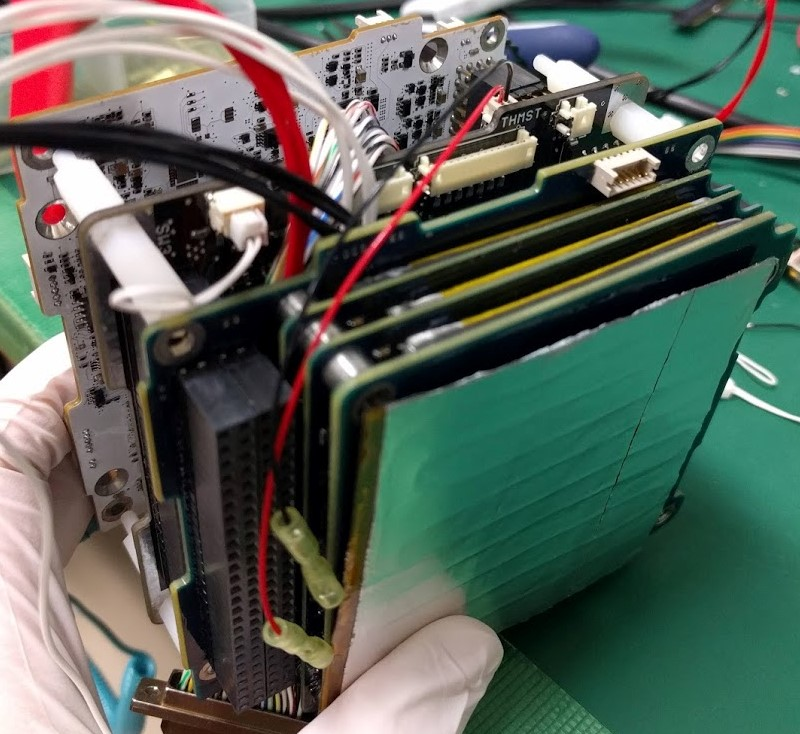
\includegraphics[width=0.5\linewidth]{./03/fig/heater.jpg}
		\caption{Cell level protection circuit schematic 転載}
		\label{cell_p}
	\end{center}
\end{figure}

\subsection{CIB電源系}

\begin{figure}[htbp]
	\begin{minipage}{0.5\hsize}
		\begin{center}
			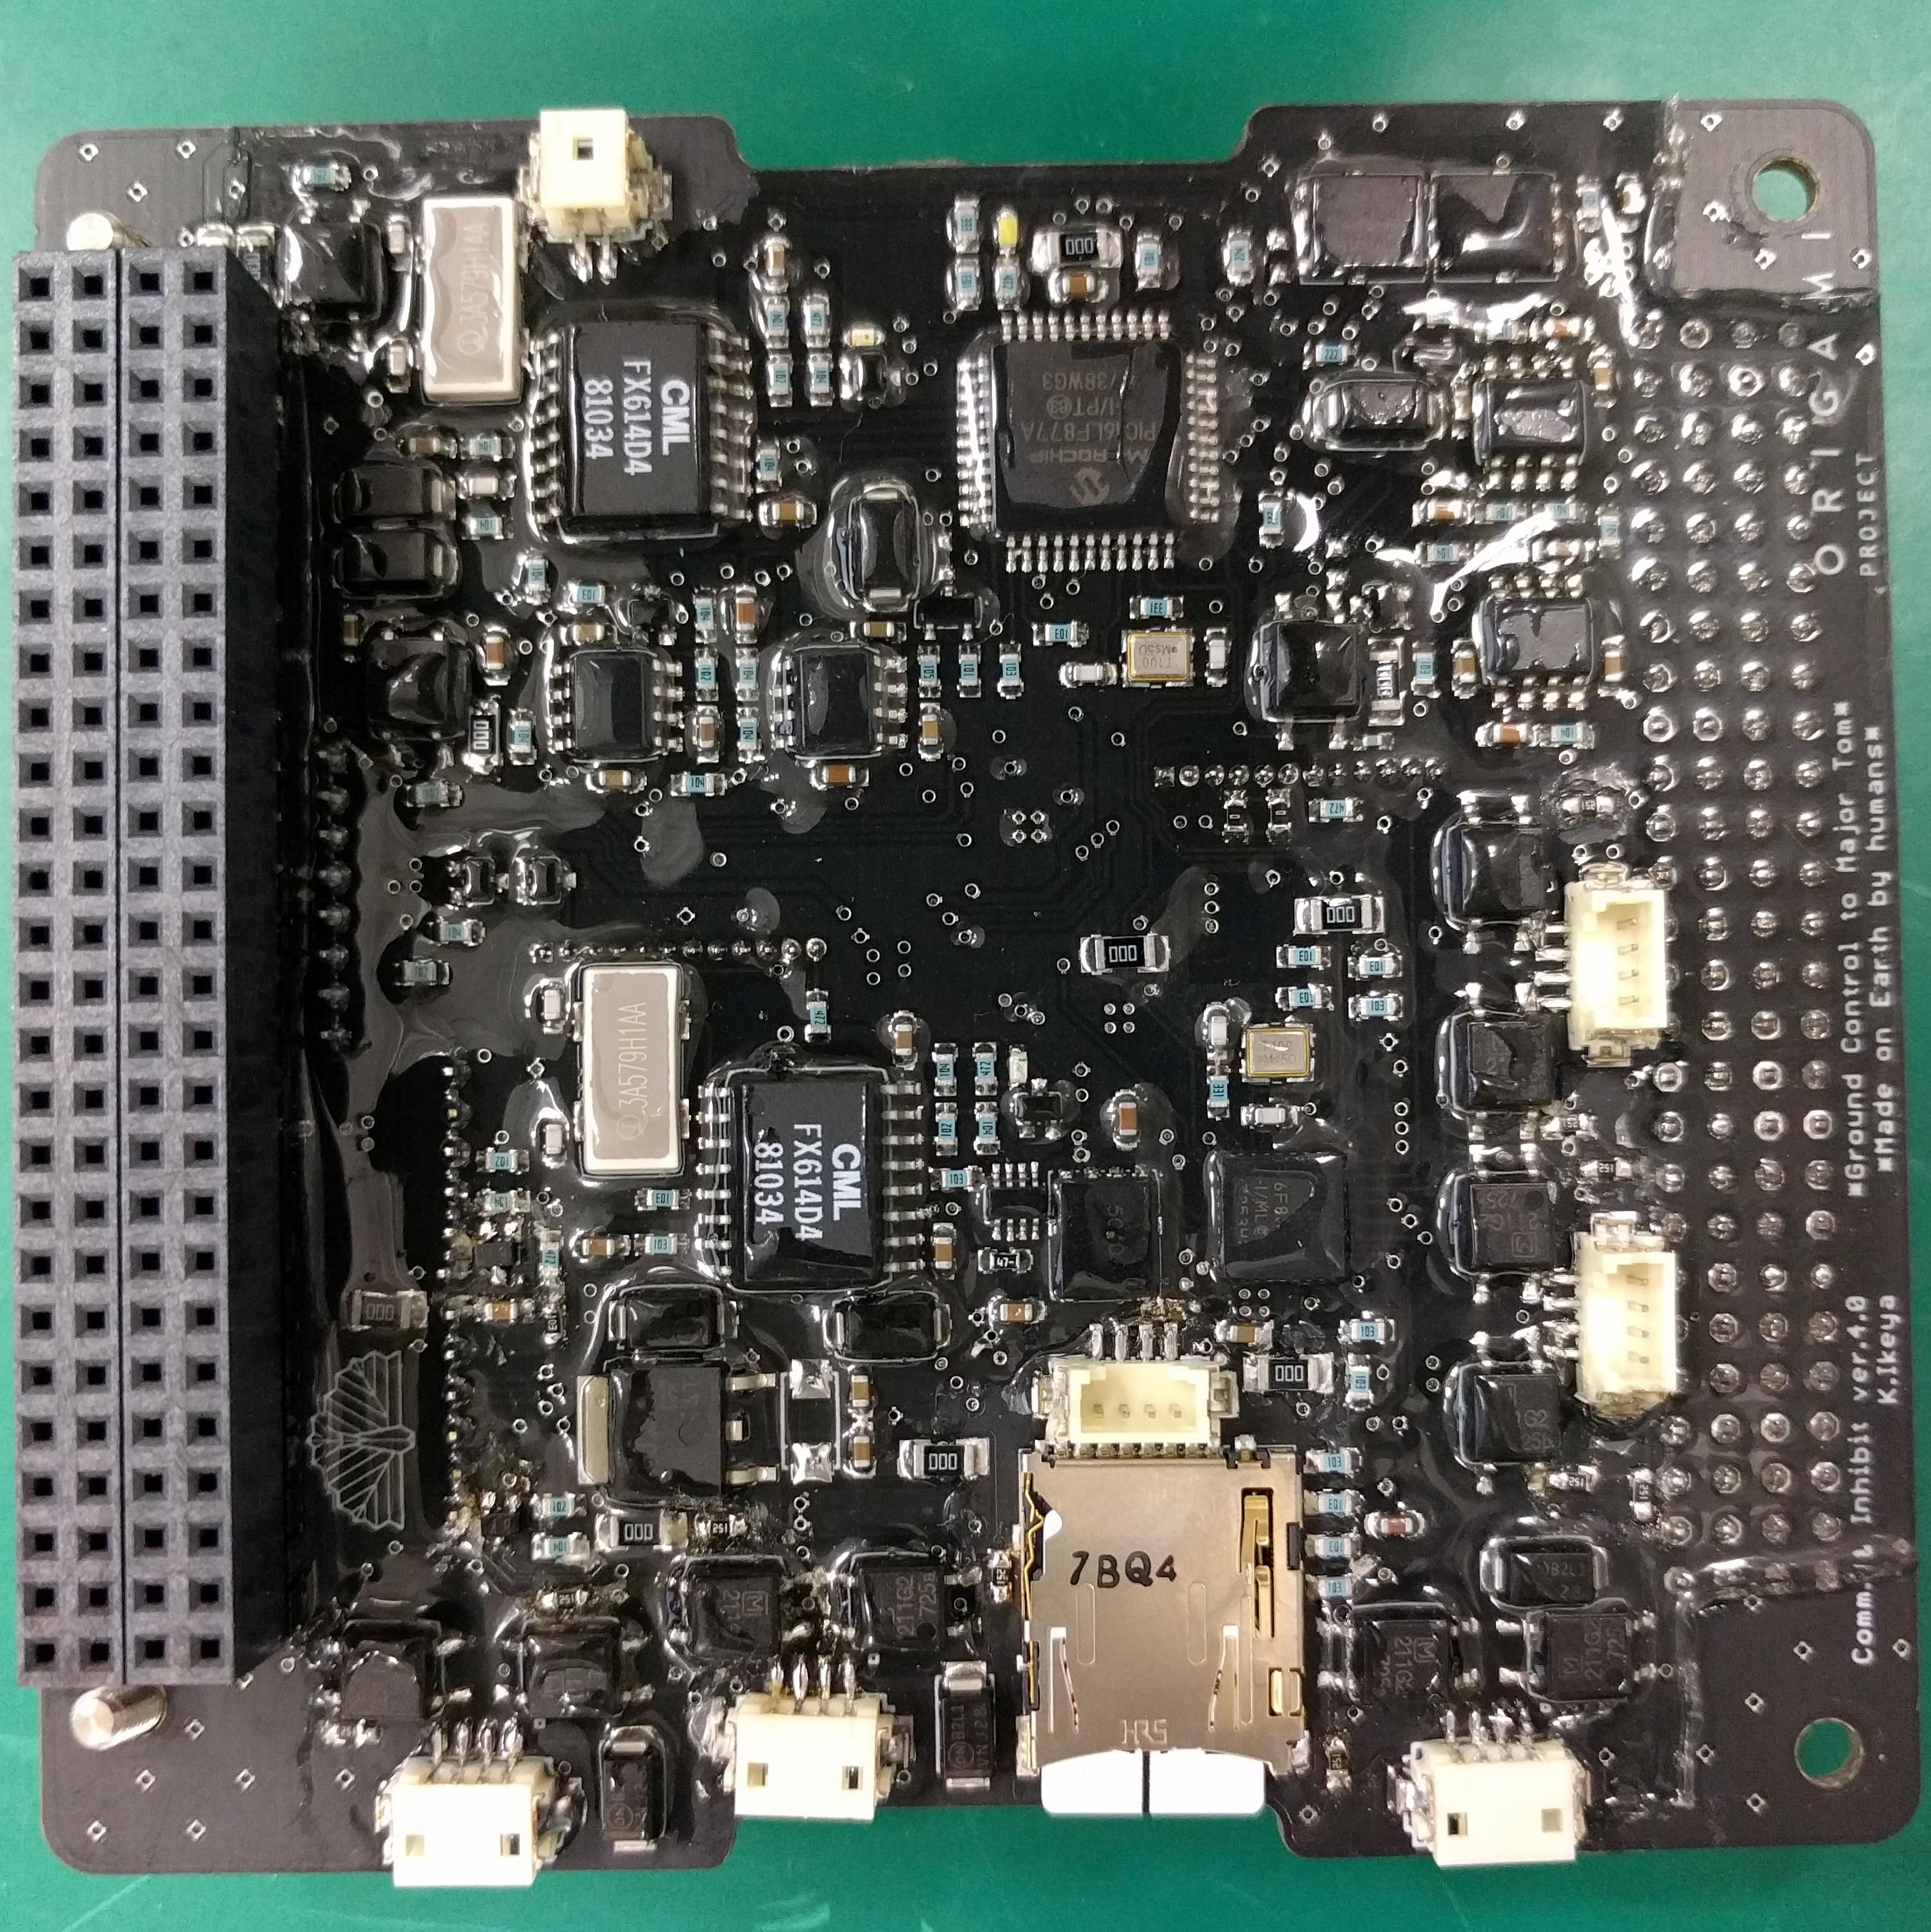
\includegraphics[width=0.7
			\linewidth]{./03/fig/CIB_1.jpg}
		\end{center}
	\end{minipage}
	\begin{minipage}{0.5\hsize}
		\begin{center}
			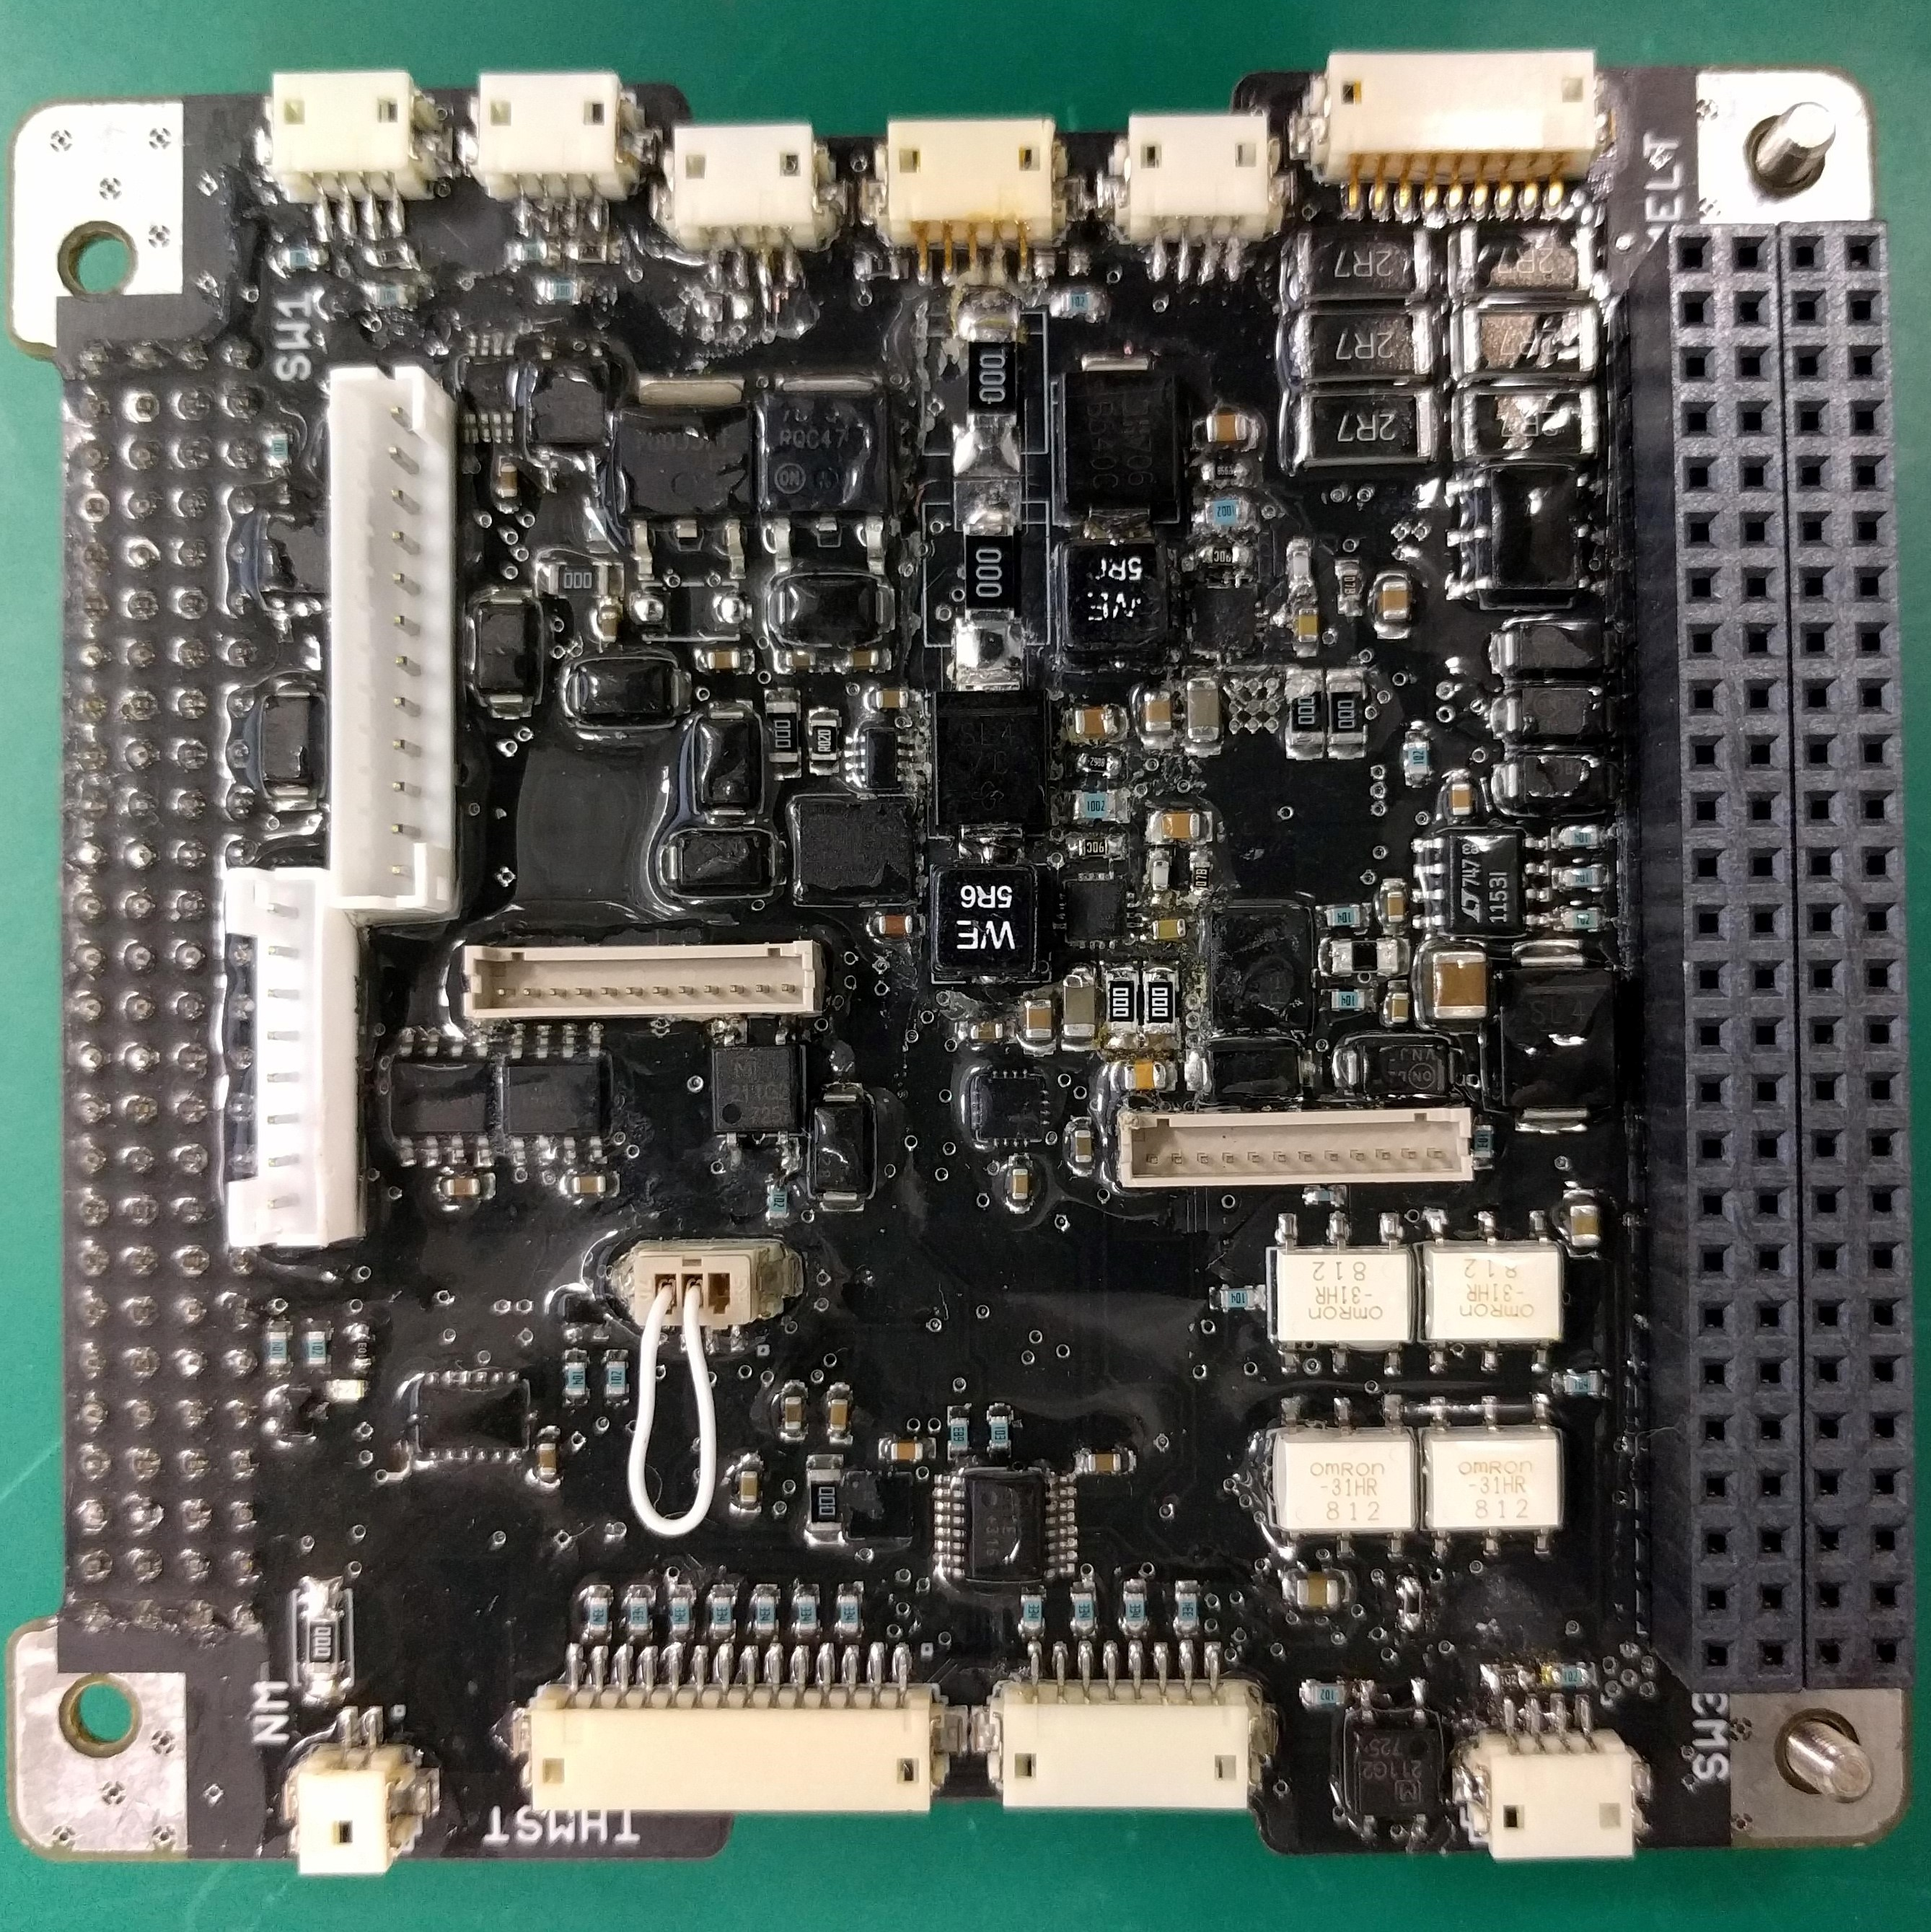
\includegraphics[width=0.7\linewidth]{./03/fig/CIB_2.jpg}
		\end{center}
	\end{minipage}\\		
	\begin{center}
		\caption{CIB}
	\end{center}
\label{CIB}
\end{figure}

\subsubsection{インヒビット回路}
イプシロンロケット
ACX-11007「小型副衛星の安全設計手引き制定初版」を参考に
要求により

以下のハザードを設けられた
これらのハザードに対応するために
3インヒビット回路を設けた.

購入品ではこれらの要求を満たせなかったため新たに

Battery-EPS間に新たに

ただし現在は3インヒビット要求を満たすバッテリがClyde Space社から新たに発売されている

\begin{figure}[htbp]
	\begin{center}
		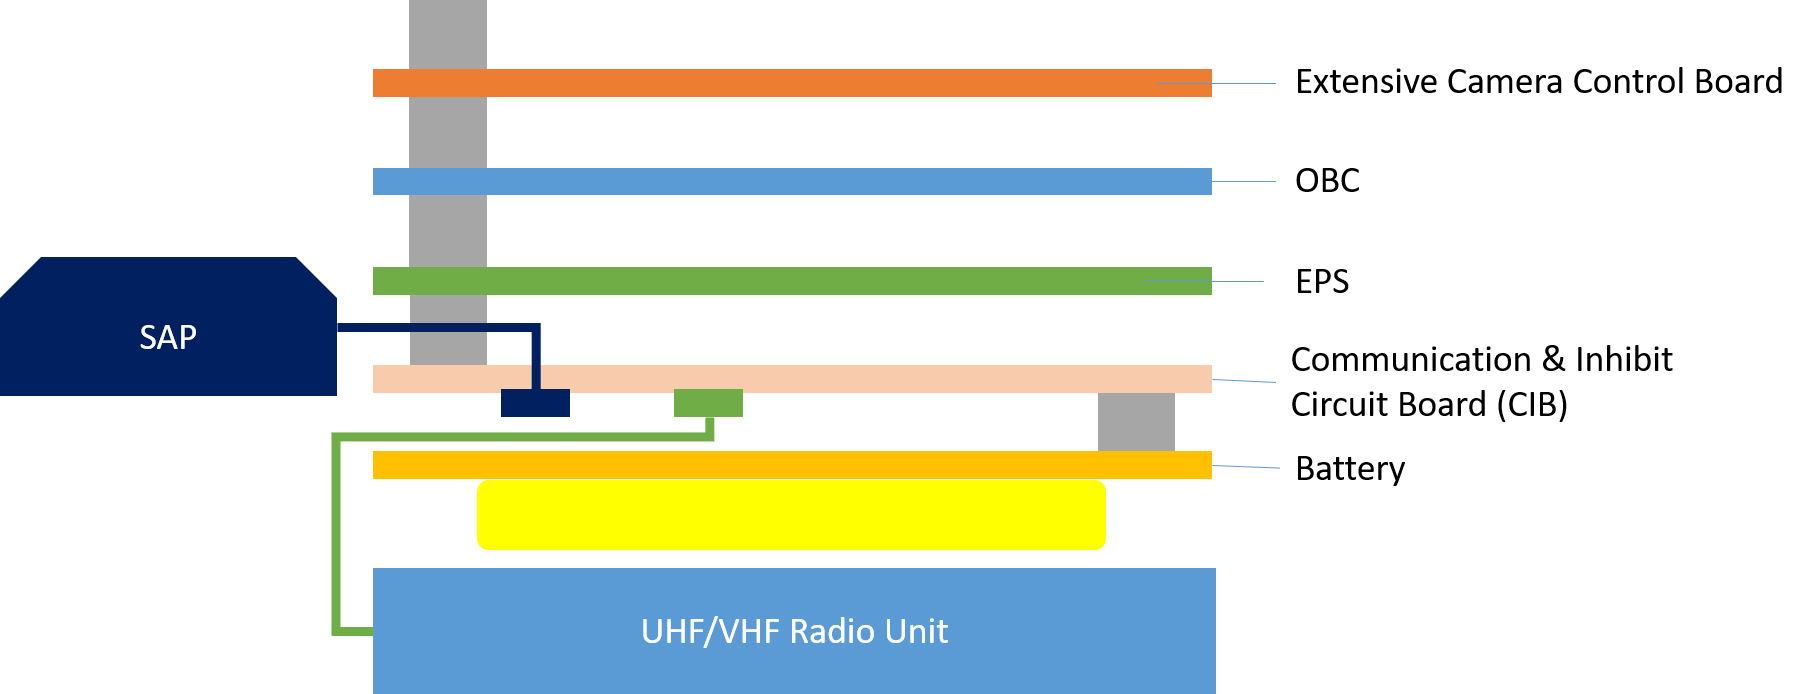
\includegraphics[width=0.7\linewidth]{./03/fig/cib_position.png}
		\caption{Cell level protection circuit schematic 転載}
		\label{fig3_1_cibposi}
	\end{center}
\end{figure}
インヒビット回路の回路図は

のようになっている

SAP-EPS間の遮断


リターン側のMOSFETをBack to Back
で双方向
実際には片方のみで問題ない
HOT側のPhotoMOSは
型番


これらのIC選定の基準として

またP-chanel MOS

回路の簡易化のために
ただしMOS
内部抵抗は概して小さい
これらのIC動作の不具合は致命的であるため
実際には並列に接続した

\begin{figure}[htbp]
	\begin{center}
		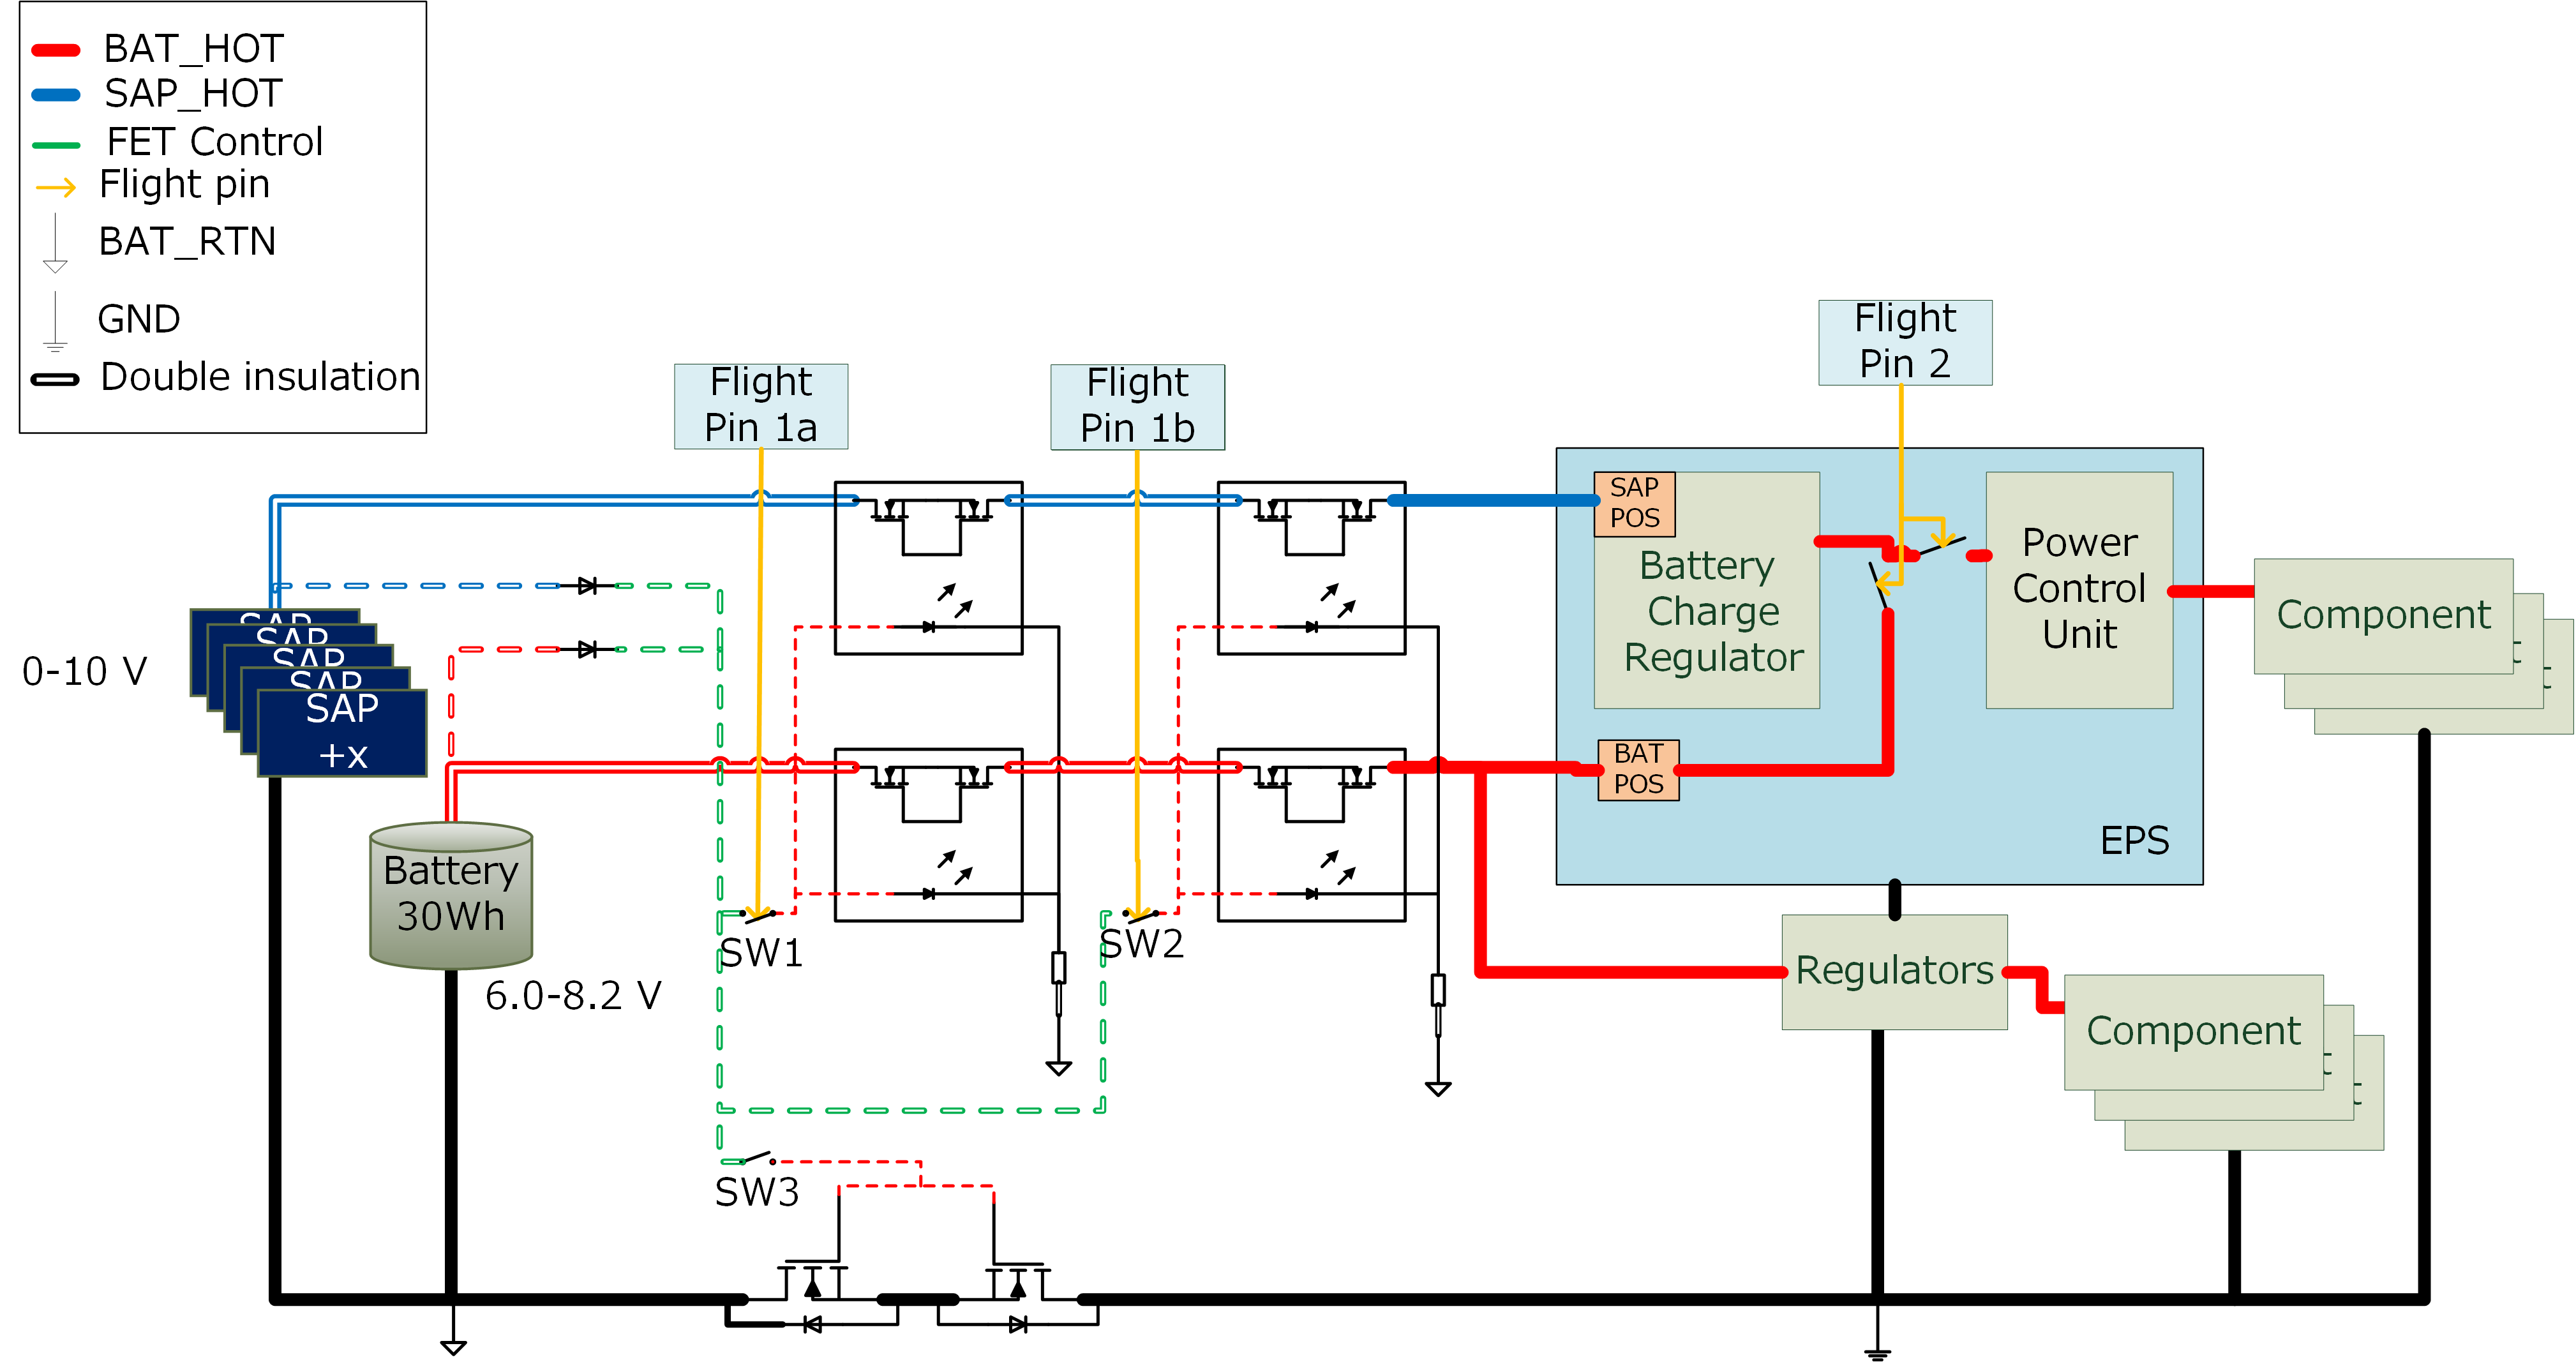
\includegraphics[width=0.9\linewidth]{./03/fig/inhibit_diagram_2.png}
		\caption{Integrated EPS and Battery Protection Architecture 転載}
		\label{fig3_1_inhibit_d}
	\end{center}
\end{figure}

\subsubsection{フライトピン}
衛星のハンドリング中




\subsubsection{CIB内電源回路}
通信用マイコンであるRXCOBC,TXCOBCはミッション開始から終了までほぼすべての期間で起動している必要がある.EPSから供給されるコンポーネントの一括on/offを可能にするためにこれらの電源系はEPS基板とは別に新たに設け,EPS電源が入っていない状態においても衛星として最低限の役割が機能するように設計した.




そこで新たな電源回路をCIB内に設けた.RXCOBC,TXCOBCの電源である3.3 V系は軌道上での故障が許されない
そこで一般的に効率の良いスイッチングレギュレータ,ではなく信頼性の高い三端子レギュレータを使用した.さらにレギュレータが1つ動作しなかった場合に備えて二つのレギュレータを並列で繋いだ.

参考文献


\begin{figure}[htbp]
	\begin{center}
		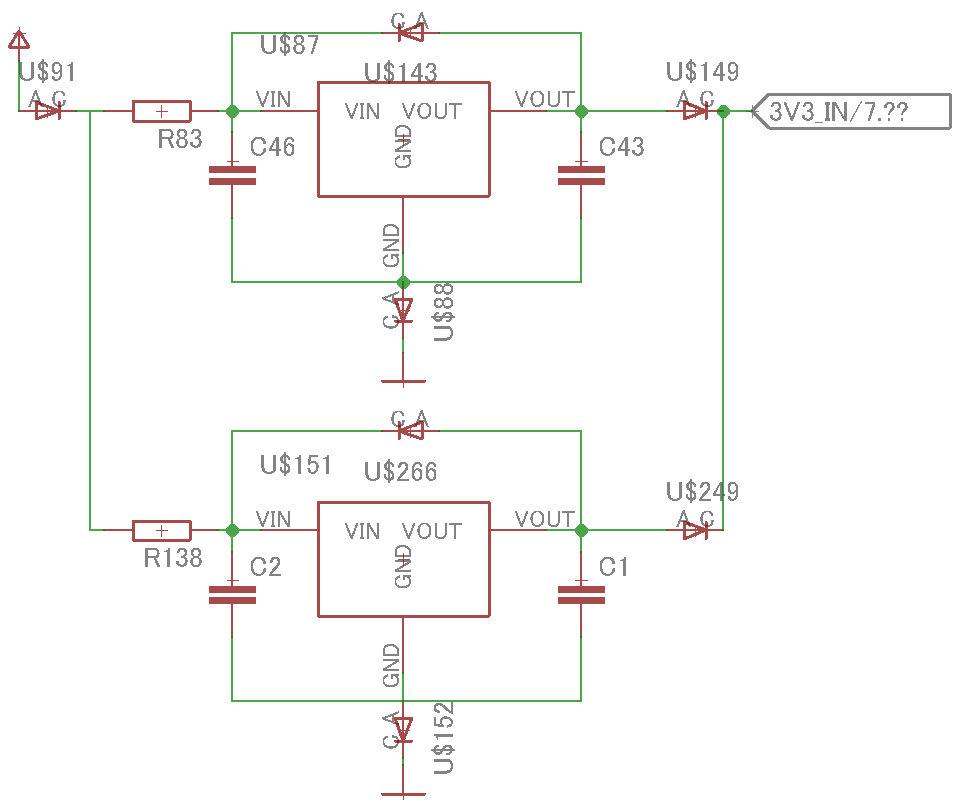
\includegraphics[width=0.6\linewidth]{./03/fig/3V3.png}
		\caption{Integrated EPS and Battery Protection Architecture 転載}
		\label{fig3_1_inhibit_d}
	\end{center}
\end{figure}

およびUHF/VHF無線機


また5.8GHz送信を行う際の突入電流が非常に大きくEPSの
保護機能が働いてしまうために12V系も新たにCIB上に設計した


12V系は
突入電流が
購入EPSの

そこで新たにDC-DCコンバータ

これらは二重に

さらに過電流対策

放射線試験によるICの放射線耐性を




\subsection{EPS}
EPSは

を購入した
\begin{figure}[htbp]
	\begin{center}
		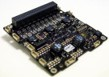
\includegraphics[width=0.5\linewidth]{./03/fig/eps.jpg}
		\caption{EPS}
		\label{eps}
	\end{center}
\end{figure}

\subsection{ミッション部電源系}
ミッション部電源系は
Raspberry Pi
が受け取ったUART信号により
スイッチのON/OFFを切り替える
\ref{}にて
後述する


